\chapter{Arhitektura i dizajn sustava}
		
		\textbf{\textit{dio 1. revizije}}\\

		\textit{ Potrebno je opisati stil arhitekture te identificirati: podsustave, preslikavanje na radnu platformu, spremišta podataka, mrežne protokole, globalni upravljački tok i sklopovsko-programske zahtjeve. Po točkama razraditi i popratiti odgovarajućim skicama:}
	\begin{itemize}
		\item 	\textit{izbor arhitekture temeljem principa oblikovanja pokazanih na predavanjima (objasniti zašto ste baš odabrali takvu arhitekturu)}
		\item 	\textit{organizaciju sustava s najviše razine apstrakcije (npr. klijent-poslužitelj, baza podataka, datotečni sustav, grafičko sučelje)}
		\item 	\textit{organizaciju aplikacije (npr. slojevi frontend i backend, MVC arhitektura) }		
	\end{itemize}

	
		

		

				
		\section{Baza podataka}
			
			\textbf{\textit{dio 1. revizije}}\\
			
		\textit{Potrebno je opisati koju vrstu i implementaciju baze podataka ste odabrali, glavne komponente od kojih se sastoji i slično.}
		
			\subsection{Opis tablica}
			

				\textit{Svaku tablicu je potrebno opisati po zadanom predlošku. Lijevo se nalazi točno ime varijable u bazi podataka, u sredini se nalazi tip podataka, a desno se nalazi opis varijable. Svjetlozelenom bojom označite primarni ključ. Svjetlo plavom označite strani ključ}
				
				\begin{longtabu} to \textwidth {|X[6, l]|X[6, l]|X[20, l]|}
					
					\hline \multicolumn{3}{|c|}{\textbf{korisnik - ime tablice}}	 \\[3pt] \hline
					\endfirsthead
					
					\hline \multicolumn{3}{|c|}{\textbf{korisnik - ime tablice}}	 \\[3pt] \hline
					\endhead
					
					\hline 
					\endlastfoot
					
					\cellcolor{LightGreen}IDKorisnik & INT	&  	Lorem ipsum dolor sit amet, consectetur adipiscing elit, sed do eiusmod tempor incididunt ut labore et dolore magna aliqua. Ut enim ad minim veniam 	\\ \hline
					korisnickoIme	& VARCHAR &   	\\ \hline 
					email & VARCHAR &   \\ \hline 
					ime & VARCHAR	&  		\\ \hline 
					\cellcolor{LightBlue} primjer	& VARCHAR &   	\\ \hline 
					
					
				\end{longtabu}
			
			\begin{longtabu} to \textwidth {|X[8, l]|X[6, l]|X[20, l]|}
				
				\hline \multicolumn{3}{|c|}{\textbf{Uredaj}}	 \\[3pt] \hline
				\endfirsthead
				
				\hline \multicolumn{3}{|c|}{\textbf{Uredaj}}	 \\[3pt] \hline
				\endhead
				
				\hline 
				\endlastfoot
				
				\cellcolor{LightGreen}id & INT	&  Id uređaja u praonici.	\\ \hline
				ime	& VARCHAR &   Ime uređaja (npr. Perilica1, Sušilica5...).	\\ \hline 
				vrsta & BOOLEAN &  Vrsta uređaja(perilica ili sušilica). Ako je perilica, vrijednost je 1, a ako je sušilica, vrijednost je 0.\\ \hline 
				
				
			\end{longtabu}
		
			\begin{longtabu} to \textwidth {|X[8, l]|X[6, l]|X[20, l]|}
				
				\hline \multicolumn{3}{|c|}{\textbf{RezerviraniTermin}}	 \\[3pt] \hline
				\endfirsthead
				
				\hline \multicolumn{3}{|c|}{\textbf{RezerviraniTermin}}	 \\[3pt] \hline
				\endhead
				
				\hline 
				\endlastfoot
				
				\cellcolor{LightGreen}termin & TIMESTAMP	&  	Datu rezerviranog termina u praonici i vrijeme početka. 	\\ \hline
				\cellcolor{LightGreen}idUredaj	& INT &  Id uređaja kojeg rezerviramo u terminu. 	\\ \hline 
				cijena & FLOAT &  Cijena usluge koju korisnik plaća (pranje ili sušenje). \\ \hline 
				biljeska & VARCHAR	& Korisnik može ostaviti bilješku zaposleniku (koja odjeća ne ide u sušilicu ili kašnjenje). Bilješku može mijenjati prije termina i za vrijeme termina.  		\\ \hline 
				placeno & BOOLEAN	& Korisnik bira hoće li platiti termin online ili uživo. U slučaju plaćanja online, nakon potvrde plaćanja, vrijednost je 1. Ako korisnik želi platiti uživo, zaposlenik praonice potvrđuje plaćanje i postavlja vrijednost u 1. Inače je vrijednsot 0.		\\ \hline 
				posudjenaKosara & BOOLEAN	& Korisnik može posuditi jednu košaru iz praonice. 	\\ \hline 
				\cellcolor{LightBlue} idKorisnik	& INT &  Id korisnika koji je rezervirao termin. 	\\ \hline 
				\cellcolor{LightBlue} idZaposlenik	& INT &  Id zaposlenika koji radi za vrijeme rezerviranog termina. 	\\ \hline
				
			\end{longtabu}
		
			\begin{longtabu} to \textwidth {|X[8, l]|X[6, l]|X[20, l]|}
				
				\hline \multicolumn{3}{|c|}{\textbf{Korisnik}}	 \\[3pt] \hline
				\endfirsthead
				
				\hline \multicolumn{3}{|c|}{\textbf{Korisnik}}	 \\[3pt] \hline
				\endhead
				
				\hline 
				\endlastfoot
				
				\cellcolor{LightGreen}id & INT	&  Id korisnika.	\\ \hline
				ime	& VARCHAR &   Ime korisnika.	\\ \hline 
				prezime	& VARCHAR &   Prezime korisnika.	\\ \hline
				lozinka	& VARCHAR &   Lozinka korisničkog računa.	\\ \hline
				email	& VARCHAR &   Jedinstveni email korisnika.	\\ \hline
				aktivan & BOOLEAN &  Svi korisnici čije registracije su potvrđene od zaposlenika su aktivni. Administrator može blokirati korisnika i promijeniti zastavicu u 0. Neaktivni korisnici nemaju pristup uslugama praonice.\\ \hline 
				ocjena & FLOAT &  Aritmetička sredina svih dobivenih ocjena za pojedinog djelatnika.\\ \hline 
				zaposlenik & BOOLEAN &  Korisnici mogu biti i zaposlenici. Ako je korisnik ujedno i zaposlenik vrijednost zastavice je 1. Zaposlenici imaju više ovlasti od običnih korisnika.\\ \hline 
			
				
				
			\end{longtabu}
		
			\begin{longtabu} to \textwidth {|X[8, l]|X[6, l]|X[20, l]|}
				
				\hline \multicolumn{3}{|c|}{\textbf{Objava}}	 \\[3pt] \hline
				\endfirsthead
				
				\hline \multicolumn{3}{|c|}{\textbf{Objava}}	 \\[3pt] \hline
				\endhead
				
				\hline 
				\endlastfoot
				
				\cellcolor{LightGreen}id & INT	&  Id objave.	\\ \hline
				
				
				slika	& BYTEA &   Slika priložena uz objavu.	\\ \hline 
				tekst	& VARCHAR &   Tekst objave.	\\ \hline
				datumObjave	& DATE &  Datum objavljivanja objave.	\\ \hline
				LF	& BOOLEAN &   Ako je vrijednost zastavice, objava se prikazuje na "LostAndFound" stranici. 	\\ \hline
				\cellcolor{LightBlue} idZaposlenik	& INT &  Id zaposlenika koji radi za vrijeme rezerviranog termina. 	\\ \hline		
						
				
				
			\end{longtabu}
		
			\begin{longtabu} to \textwidth {|X[8, l]|X[6, l]|X[20, l]|}
				
				\hline \multicolumn{3}{|c|}{\textbf{Recenzije}}	 \\[3pt] \hline
				\endfirsthead
				
				\hline \multicolumn{3}{|c|}{\textbf{Recenzije}}	 \\[3pt] \hline
				\endhead
				
				\hline 
				\endlastfoot
				
				\cellcolor{LightGreen}id & INT	&  Id recenzije.	\\ \hline
				\cellcolor{LightBlue} idKorisnik	& INT &  Id korisnika koji je ostavio recenziju. 	\\ \hline
				\cellcolor{LightBlue} idZaposlenik	& INT &  Id recenziranog zaposlenika. 	\\ \hline
				recenzija	& VARCHAR &   Tekst recenzije.	\\ \hline
				ocjena	& INT & Ocjena zaposlenika od 1 do 5.	\\ \hline
				
			\end{longtabu}
			
			\begin{longtabu} to \textwidth {|X[8, l]|X[6, l]|X[20, l]|}
				
				\hline \multicolumn{3}{|c|}{\textbf{Praonica}}	 \\[3pt] \hline
				\endfirsthead
				
				\hline \multicolumn{3}{|c|}{\textbf{Praonica}}	 \\[3pt] \hline
				\endhead
				
				\hline 
				\endlastfoot
				
				\cellcolor{LightGreen}datum & DATUM	&  Trenutni datum.	\\ \hline
				pocetakRada	& TIME &   Početak radnog vremena.	\\ \hline
				krajRada	& TIME & Kraj radnog vremena.	\\ \hline
				pauza	& TIME & Početak pauze.	\\ \hline
				pranjeCijena	& FLOAT & Cijena jednog pranja.	\\ \hline
				susenjeCijena	& FLOAT & Cijena jednog sušenja.	\\ \hline
				
				
			\end{longtabu}
			
			
			\subsection{Dijagram baze podataka}
				\textit{ U ovom potpoglavlju potrebno je umetnuti dijagram baze podataka. Primarni i strani ključevi moraju biti označeni, a tablice povezane. Bazu podataka je potrebno normalizirati. Podsjetite se kolegija "Baze podataka".}
				
				\begin{figure}[H]
					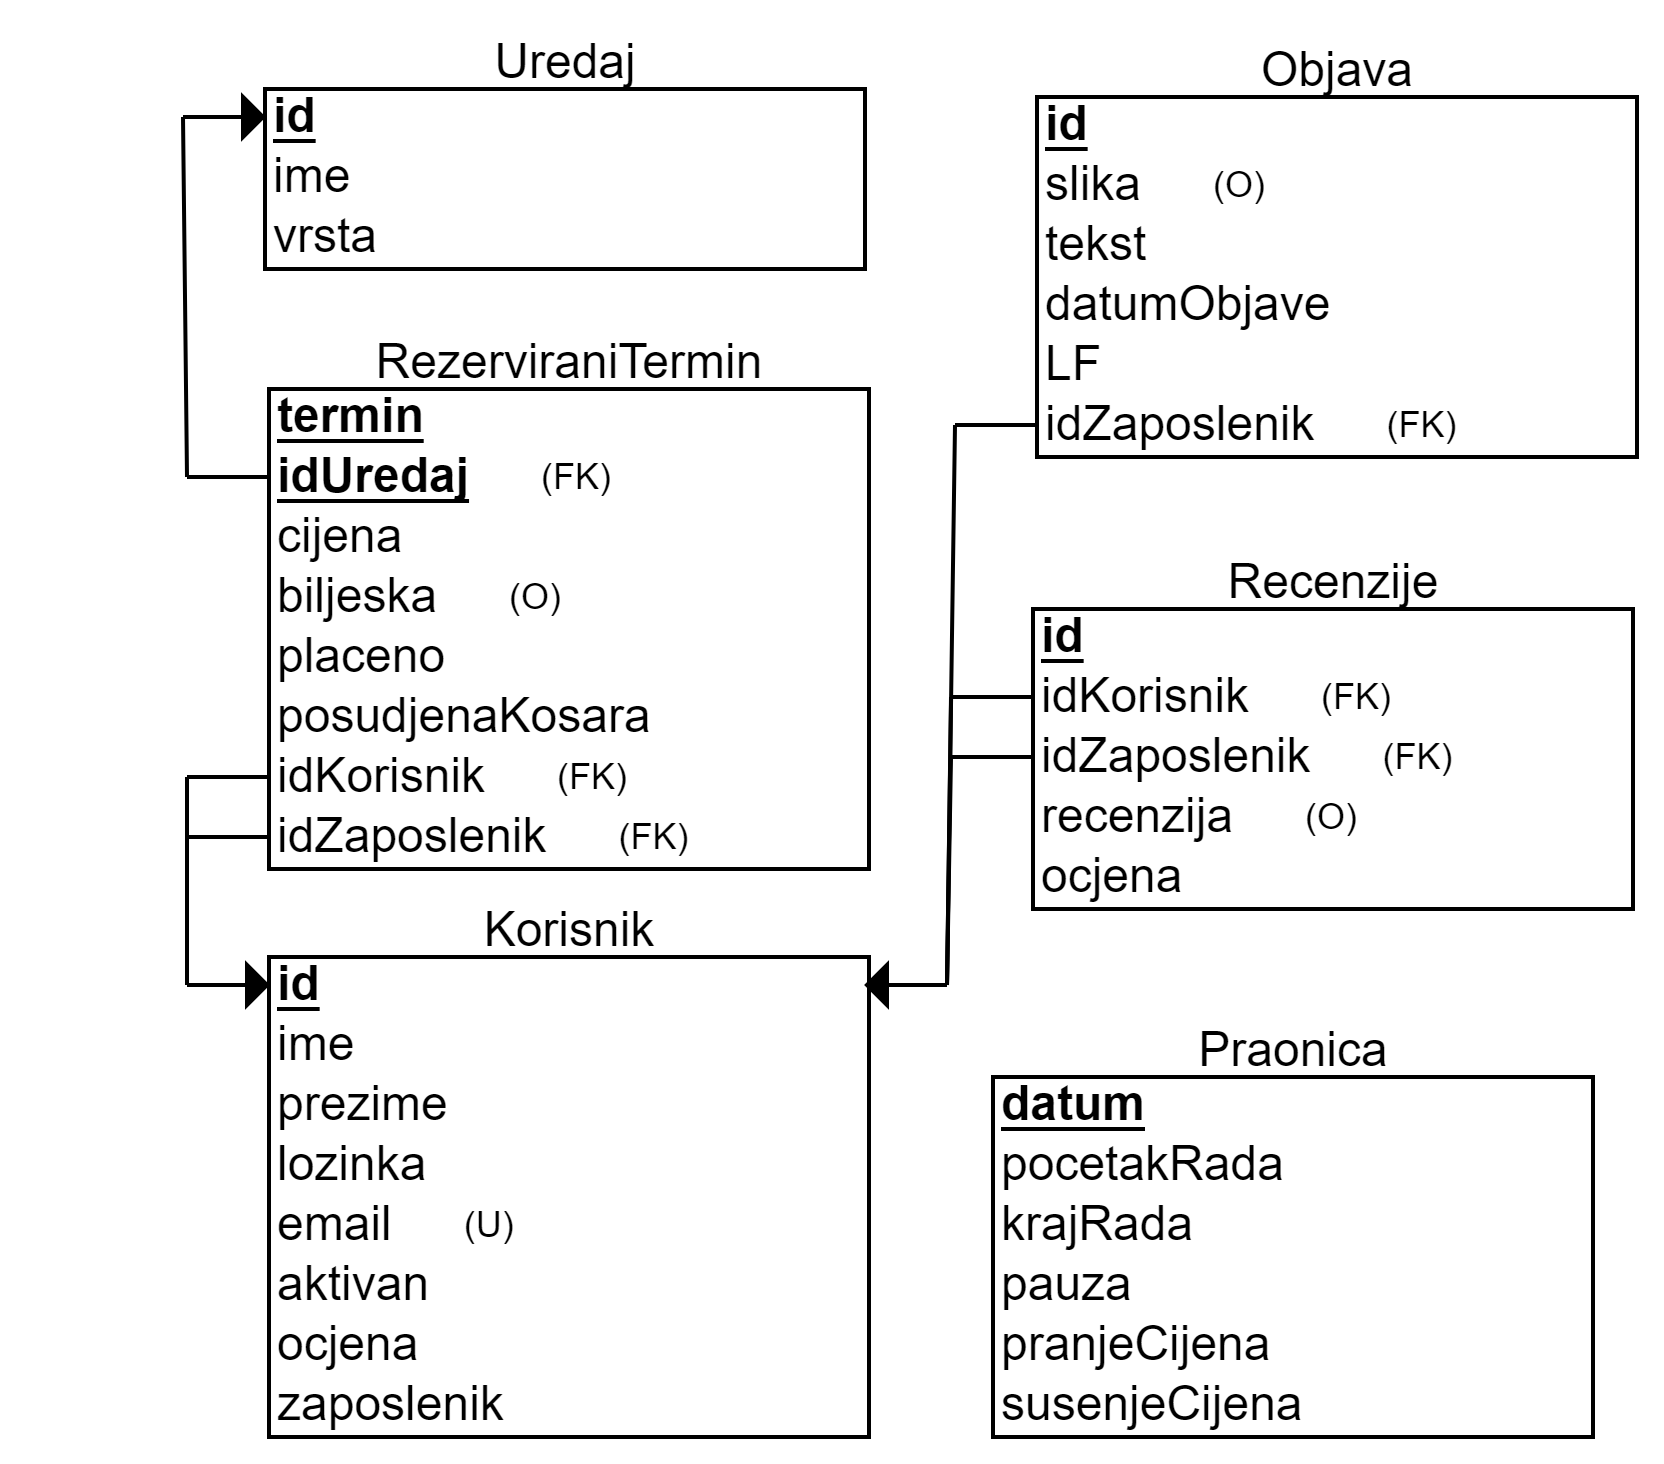
\includegraphics[scale=0.2]{slike/BAZA.PNG} %veličina slike u odnosu na originalnu datoteku i pozicija slike
					\centering
					\caption{Relacijska shema baze podataka}
					\label{fig:promjene}
				\end{figure}
			\eject
			
			
		\section{Dijagram razreda}
		
			\textit{Potrebno je priložiti dijagram razreda s pripadajućim opisom. Zbog preglednosti je moguće dijagram razlomiti na više njih, ali moraju biti grupirani prema sličnim razinama apstrakcije i srodnim funkcionalnostima.}\\
			
			\textbf{\textit{dio 1. revizije}}\\
			
			\textit{Prilikom prve predaje projekta, potrebno je priložiti potpuno razrađen dijagram razreda vezan uz \textbf{generičku funkcionalnost} sustava. Ostale funkcionalnosti trebaju biti idejno razrađene u dijagramu sa sljedećim komponentama: nazivi razreda, nazivi metoda i vrste pristupa metodama (npr. javni, zaštićeni), nazivi atributa razreda, veze i odnosi između razreda.}\\
			
			\textbf{\textit{dio 2. revizije}}\\			
			
			\textit{Prilikom druge predaje projekta dijagram razreda i opisi moraju odgovarati stvarnom stanju implementacije}
			
			
			
			\eject
		
		\section{Dijagram stanja}
			
			
			\textbf{\textit{dio 2. revizije}}\\
			
			\textit{Potrebno je priložiti dijagram stanja i opisati ga. Dovoljan je jedan dijagram stanja koji prikazuje \textbf{značajan dio funkcionalnosti} sustava. Na primjer, stanja korisničkog sučelja i tijek korištenja neke ključne funkcionalnosti jesu značajan dio sustava, a registracija i prijava nisu. }
			
			
			\eject 
		
		\section{Dijagram aktivnosti}
			
			\textbf{\textit{dio 2. revizije}}\\
			
			 \textit{Potrebno je priložiti dijagram aktivnosti s pripadajućim opisom. Dijagram aktivnosti treba prikazivati značajan dio sustava.}
			
			\eject
		\section{Dijagram komponenti}
		
			\textbf{\textit{dio 2. revizije}}\\
		
			 \textit{Potrebno je priložiti dijagram komponenti s pripadajućim opisom. Dijagram komponenti treba prikazivati strukturu cijele aplikacije.}